\documentclass[12pt]{article}
\usepackage[hmargin=1in,vmargin=1in]{geometry}
\usepackage{setspace}
\usepackage{graphicx}
\usepackage{fixme}

\title{An Open Source Data Storage and Visualization Backend for Experimental
Data} 
\author{K. Nielsen, T. Andersen, R. Jensen, J.H. Nielsen and I. Chorkendorff}
% Eller hvilken rækkefølge vi nu lyster... 

\date{\today}

\renewcommand{\rmdefault}{phv} % Font setup (Arial)
\renewcommand{\sfdefault}{phv} % Font setup (Arial)

\begin{document}
\doublespacing % Double spacing, \singlespacing \onehalfspacing setstretch{x}
\maketitle

\begin{abstract}
In this article the creation of a flexible Free and Open Source
Software (FOSS) system for data logging and presentation will be
described. The flexibility of the system originates from the use
primarily of FOSS and from the structure of the system. This structure
consists of three parts, a data server, data logging clients and a
data presentation website. The logging of data from independent
clients leads to high resilience to equipment failure, while the
central storage of data dramatically ease backup and data
exchange. The data stored consist both of specific measurements and of
continuously logged system parameters. The latter is crucial to a
variety of automation and surveillance features and 3 cases of such
features are described; monitoring system health, getting the status of
the equipment during experiments with long durations and implementing
instant alarms in the event of cooling water failure.
\end{abstract}

\section{Introduction}
In every experimental laboratory the need for acquisition and subsequent
logging of data is of essential importance. Typically, logbooks, either in
electronic or paper form, is used to organize large amounts of data and note
down experimental parameters. The acquired data from a given experiment is
typically stored locally on the laboratory computer. The data is often acquired
in highly specialized proprietary software in proprietary formats. When working
with different experimental systems across several computers with different
software suites, operating systems etc. the exchange of acquired data is
cumbersome and difficult due to the nature of proprietary formats.

A solution to simplify and make data exchange easier across several platforms
is to store all acquired experimental data on a centralized server. This has a
number of attractive features. Firstly, by storing data on a centralized server
backup of all experimental data enormously simplified. Secondly, the data is
stored in a standardized and open format which allows easy export of the data
to any platform or software source.

The access to a centralized point of storage for experimental data also allows
for real-time continuous logging of various parameters used as indicators for
system health. Critical system parameters can hence be monitored and used to
trigger alarms when these fall out of specified ranges. Furthermore, the
logging of experimental setup parameters continuously enables access to these
values at any previous point in time.

A centralized storage of data can be accomplished in many ways. However, in
experimental laboratories where large amounts of data are recorded a database
is an obvious choice for storage. Here we present a totally open source system
consisting of data acquisition, storage in a MySQL database and a comprehensive
display module including simple data treatment algorithms which is open source
software.



\section{System description}
The system is based on Python, PHP and HTML/CSS integrated with Linux servers
running MySQL and/or Apache (LAMP setup). Experimental data is acquired on the
user side and subsequently stored in the MySQL database. Python, PHP and
HTML/CSS is used to extract data from the database and present them to the end
user in a simple user interactive webinterface for data visualization and
manipulation. Python was primarily chosen due to its tight integration with
scientific packages which makes data analysis and treatment more
convenient\cite{Cahn2007}. PHP and HTML/CSS is used to display data in
standardized formats suitable for web browsers and process input from the user.
The combination of PHP and HTML/CSS to store data and process user input from
webpages is very flexible and has proven successful in other parts of the
scientific community\cite{Crane2008}.

The system consists of three logically separate components as illustrated in
Figure~\ref{fig:system_overview}; 1) the equipment component where all
communication with apparatus and acquisition of data is performed 2) the
servers which consist of the MySQL server that stores the acquired data from
experiments and the webserver (Apache) which interacts and presents the user with data
retrieved from the database and 3) the user component which is made up of the
clints whishing to access the data. \begin{figure}
 \begin{center}
 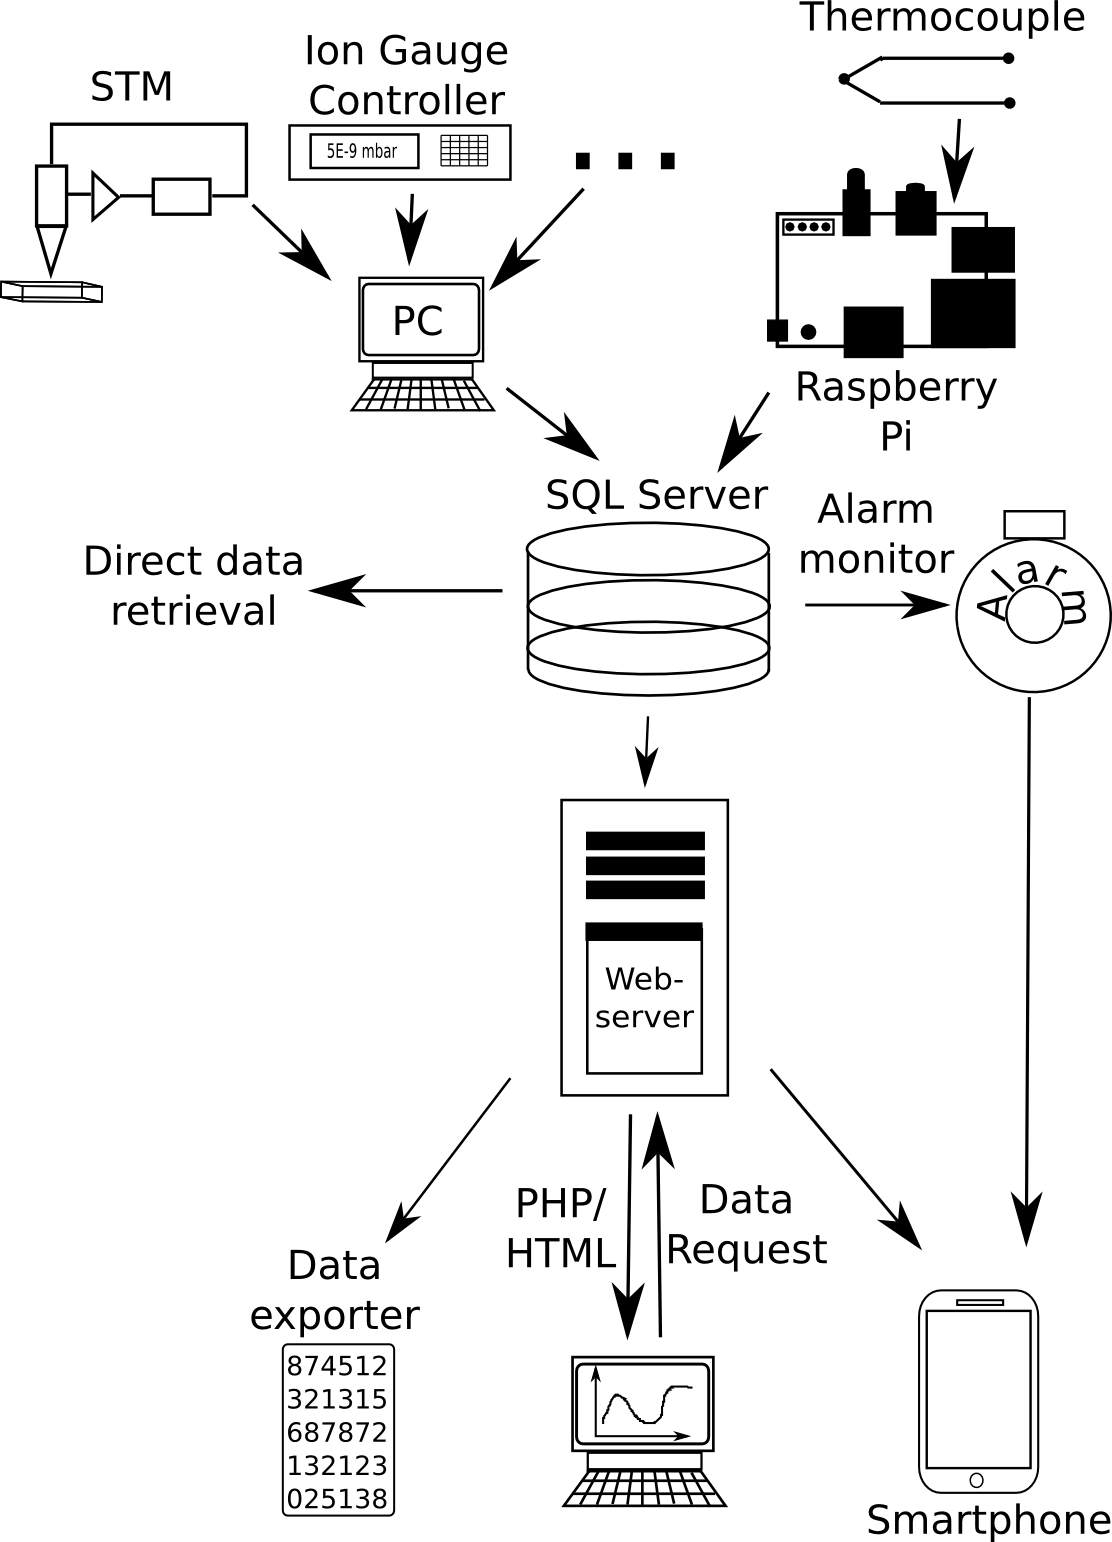
\includegraphics[width=10cm]{system_overview.png}
 \caption{
   A schematic representation of the structure of data handling system.
   \label{fig:system_overview}
 } 
 \end{center}
\end{figure}

The system is highly modular meaning the servers can accept data from a range
of different sources. In the current setup equipment interfaced with RS232,
GPIB, USB, analog/digital data acquisition cards standards are logged to the
MySQL database. The user can furthermore use programs written in a wide variety
of languages. As a testimony to this, software written in both LabView and
Python are used to save data to the database. How the integration with the
server and subsequent storage of data in the database is performed is hence a
user determined design decision. This has a number of attractive advantages.
The user(s) can integrate existing software with the databases quickly and
without the need to rewrite any previous interface software written for
experimental setups. Furthermore, due to the flexibility of system, if online
storage in the database during acquisition is not possible due to software
limitations the data can still be saved in the database by subsequent offline
parsing of data files. This, however, still requires that the file format,
which holds the data, is specified or the data can be exported to a flat text
format from the acquisition software. 

The servers consist of a MySQL server and a webserver. All experimental data is
stored on the MySQL server and is presented to the user from the webserver. If
needed, experimental data from the MySQL server can be retrieved directly for
later analysis. The webserver runs a LAMP (Linux, Apache, MySQL,
PHP/Python) package which is used to display the data to users via
a website. Data is hence fetched from the MySQL server by the webserver and
subsequently presented for the user. To accommodate a range of users and
provide the largest flexibility the webserver displays both a standard HTML/CSS
site for desktop PCs and a mobile version suitable for tablet/smartphone users.

The webinterface, which takes user input and displays data to the user, is
also capable of routine data treatment. This can either be zoom of data,
plotting on a log scale, performing a running average, etc. The plotting is
easy extendable allowing the user to add any function necessary. In this way
the user can easily and quickly get an overview of acquired data.


\section{Data aquisition}
In large research departments any kind of data acquisition must necessarily be
strictly decentralized with several independent clients to avoid dataloss and
simplify backup of important data. This requires interfacing of many types of
computer hardware and collecting different types of data from many kinds of
instrumentation.

In practice this is achieved by formulating a set of general design goals that
will serve as computer language and hardware independent pseudo-code which
will help the process of designing a new acquisition client. The design goals
of our implementation looks as follows:

* To minimize the risk of data loss and to provide easy data-access across the
  laboratory all clients must store data for as short amount of time as
  possible before handing of the data to a central server. Preferably the data
  should be stored on the server as soon as it is acquired. For data being
  recorded over longer time-spans this means that data must be live-streamed to
  the server.

* To avoid data-loss in the event of missing network or maintenance of the
  central server all clients collecting critical data must implement a local
  queue that will temporarily hold data until the central server can again be
  accessed. The client must continuously check if the server is again available
  and as soon as possible deliver queued data to the server.

* For continuous measurements (e.g. temperature of pumps, pressure in vacuum
  chambers, etc.) data logging must be implemented in a way that ensures that
  all significant events are recorded and at the same time does not use
  excessive amounts of storage. This is typically implemented by sampling data
  in a much higher rate than they are recorded. The local client will then
  based on relevant heuristics decide whether a new data point should stored on
  the server. This is typically implemented by waiting for either a given
  relative change in the signal or a maximum time since last recording of a
  data point.
  
* For stand-alone measurements (e.g. spectrometry, electrical characterization,
  etc.) it is important to measure appropriate amounts of metadata ensuring
  that all information about the experiment is preserved. This along with
  accurate time information will ensure that questions that where not yet
  formulated at the time of the experiment can be answered in retrospect using
  the metadata along with the continuously measured parameters.
  


\section{Data storage}\label{data_storage}
Our system-design of many highly decentralized clients all pushing data
continuously to a central server means, that this server must both high
perfomance, high uptimes as well as the a flexible storage to ensure that it is
always possible to add more space if so needed. To ensure these properties of
the system, we have deliberately chosen a system as simple as possible to avoid
unneccessary complications, and to ensure that this central component can be
easily managed by the professional IT-staff of the derpartement. It is
important to realized that even though it typically is not a problem if a
single client machine somewhare in the system is temporarily down (this can
happen for many reasons in a experimental lab), it is crucial that this
particular server is handled like a real production server.

To keep the server-side of things simple, we use a relational database, in our
case MySQL\cite{mysql} which is open source and provides extremely good
performance. This MySQL server contains the entire set of data of all
experimental setups, thus it is extremely easy to backup everything by simply
doing a dump of the database with regular intervals.

Since the database is only exposed to the local network, security is not a
really a concern, however to protect agains accidential pollution of the
various setups with irrelevant data when code is exchanged between setups, each
client has its own username and password which is not part of the code
(typically it will be managed in ODBC-settings) In this way, code can flow back
and forth between setup without the risk of one setup accidentially loggin data
to other setups tables.



\section{Data access}
As mentioned in section~\ref{sec:data_extraction} it is both possible and very
easy to access data directly from the database using either direct SQL
statements or programming. This is very practical for the cases where it is
desired to perform data treatment on the data or to produce high quality
graphs. However, most of the time it is sufficient to simply look at the data
and possibly perform light data treatment. For this kind of data analysis it
would be highly impractical to write small custom pieces of software for each
kind of data that the users wish to look at. For this reason we have developed
a framework for visualization of the stored data that allows quick and easy
access to all data. The framework includes support for basic data treatment as
well as the option to plot several data sets at the same time for easy
comparison of results and to export the data to local files. An example of the
web interface used for plotting is shown in Figure~\ref{fig:webinterface}
\begin{figure}
 \begin{center}
 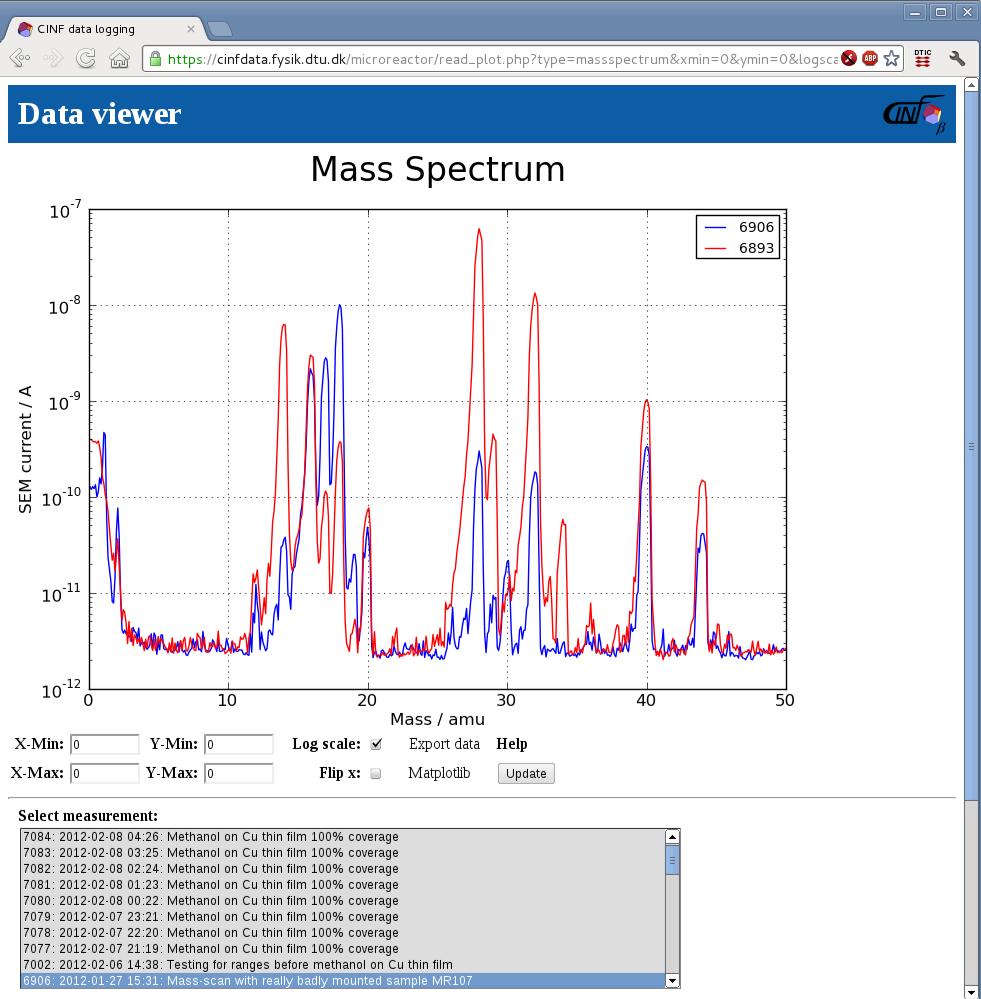
\includegraphics[width=10cm]{mass_spectra_comparison.png}
 \caption{Demonstration of the visualization interface. Data (here mass
   spectrometer data) can be plotted and compared in a web browser allowing
   easy comparison between data. \label{fig:webinterface}
 } 
 \end{center}
\end{figure}

The goal for the visualization module has not been to provide high quality
plots since this is a large task that is best solved with either dedicated
software suites or custom scripts. Instead, the quality of the plots was
targeted such that it is sufficient for different kinds of everyday use
including presentations at informal group meetings, as starting point for
discussion of data, quick data comparison etc. To realize this form of
visualization a frontend/backend topology has been implemented. The code that
handles user input is retrieved in HTML and PHP thus allowing user input to be
acquired from a web browser. The backend consists of an open source plotting
library, interface code to feed data into the plotting code and plot
preferences specific to each experimental setup. The backend is mainly written
in Python and the configuration read from a XML file unique to each setup. The
preferences file contain a settings section for each different kind of plot.
Below is shown an example of a continuously logged pressure:

\begin{verbatim} 
<!-- PRESSURE --> 
<graph type='pressure'>
  <query>SELECT unix_timestamp(time), pressure FROM pressure_SETUP
  where  time between " {from}" and "{to}" order by time</query>
  <ylabel>Pressure / Torr</ylabel>
  <title>Pressure in {setup}</title>
  <default_yscale>log</default_yscale>
  <default_xscale>dat</default_xscale>
</graph>
\end{verbatim}

The system is flexible towards choice of plotting library which is a great
advantage since different plotting libraries are optimal for different tasks.
At the moment all plotting is performed by matplotlib\cite{matplotlib}.  As a
testimony to the flexibility of the setup we have moved from our original
backend based on JpGraph\cite{jpgraph} to a backend based on matplotlib without
significant changes to the backend code. Currently, we are investigating moving
some of the display code to the JavaScript based dygraphs\cite{dygraphs} thus
producing a dual display system since this plotting library allows for real-time 
manipulation of the data using a mouse through an ordinary web browser.


\section{Cases}
The existence of this data system is paramount to several automation tasks
in our lab. Below a few examples of the use of the data system for
these purposes are described.

\subsection{Sample cleaning}
In the field of catalysis, one direction of research concerns gas
reactivity studies on the surface of single crystal samples under
Ultra High Vacuum (UHV)\fixme{Probably has been introduced before}
conditions ($\sim10^{-13}$\,mbar).

Before experiments can be performed, the sample must be properly
cleaned to ensure that no contaminants are present on the surface. The
cleaning of the surface is achieved by running a number of cleaning
cycles. Each of these cycles can take up to several hours.% and may
%include sputtering (bombardment of the surface with Ar$^+$ ions to
%peel or a part of the surface), gas exposure and heating.
Before this task was automatized, it typically required simple manual
intervention 2-4 times during a 30 to 120 minute cycle. Obviously, this
was a suboptimal solution, since a lot of time was spent, with only
small time intervals to work on other things, before the next manual
intervention.

As it is apparent that the atomization of this task lead to
significant time savings, since it allowed these cleaning cycles to
e.g.\ be run in the evening or at night. However, during the
atomization process one concerns that had to be addressed was how to
monitor the status of the cleaning and the equipment. With the data
logging system in place, all relevant parameters could easily be
continuously logged and viewed with any of the data viewing options
mentioned in section ???\fixme{insert ref}. Obviously the cleaning
program itself is responsible for the safety of the system and for
shutting it down if it goes out of boundaries. But with the continuous
logging it is a simple task to add surveillance to the cleaning that
alerts the user if it happens, which means that it can be safely
restarted if it is safe to do so. There is a specific case describing
a alarm in section \ref{sec:cooling_water_alarms}.

\subsection{Experimentation over extended time periods}

Mini-reactor example. Bla bla more exhaustive search of parameter
space for experiments with large time spans. \fixme{Finish section}

\subsection{Cooling water alarms}\label{sec:cooling_water_alarms}
*The access to a centralized point of storage for experimental data also allows
for real-time continuous logging of various parameters used as indicators for
system health. Critical system parameters can hence be monitored and used to
trigger alarms when these fall out of specified ranges. Furthermore, the
logging of experimental setup parameters continuously enables access to these
values at any previous point in time.

Several important pieces of equipment require cooling. If they loose
the cooling it will often result in equipment break down, which,
depending on the equipment, can be expensive both in repair cost and
work time lost.

In our lab the main components with critical cooling requirements are
the turbo molecular pumps that are used to maintain vacuum. We do not
have direct access to monitor the cooling water status. Therefore,
instead we mounted temperature measurements on all the pumps and log
all of the these via the data system. Then, on the server that runs
the data presentation website we added a script that fetches the
latest temperatures from the database, and if these start to climb,
sends out an alarm via email. While it was inconvenient that we were
unable to monitor the cooling water directly, this approach has the
very desirable side effect that we can now also monitor the health (to
the extent it is given by the temperature) of each pump
individually.\fixme{Decide if we want to mention this here or at all}


\section{Discussion}
\ldots

\section{Conclusions}
\ldots

\bibliographystyle{abbrv}
\bibliography{literature}

\end{document}
